% ----------------------------------------------------
% Design
% ----------------------------------------------------

\chapter{Design}\label{ch:design}

\section{Salinity Measurement Method}

The industry standard for measuring conductivity is the \gls{ctd}, which calculates salinity using conductivity, temperature and depth measurement.
\refsec{sec:salinity-measurement-techniques} discussed several alternative methods of measuring salinity.
The temperatures, environment and remote nature of the Antarctic make most of these methods difficult or impossible to use.
Additionally, the final device was required to fit through an ice core hole of $110mm$ in diameter.
While the prototype does not need to directly meet this requirement, it must be designed such that a future iteration that can.

Refractometers and chlorinity titrations have the same drawbacks as the currently used hand-held \gls{ctd}, where capturing a water sample and bringing it to the surface alters its temperature and pressure, which may alter its salinity measurement.
Microwave radiation has a lower-than-desirable accuracy.
In addition, the instruments that measure it, as well as densitometers and interferometers, are expensive and complex beyond the author's expertise.
Electromagnetic induction is one of the more promising methods because it is a nondestructive method of measuring salinity, which allows samples to be used for alternative measurements afterwards.
However, as mentioned in \refsec{subsec:salinity-from-electromagnetic-induction}, the electromagnetic and salinity relationship has yet to be thoroughly researched, and it requires a high power consumption.
This latter is a significant issue in Antarctica as storing power is challenging at very low temperatures, not to mention transporting the device.

The conductivity, temperature and depth method was determined to be the most viable for this project as it is the industry standard, and the author has significant experience with \gls{pcb} design and electronics.
Additionally, it has been proven that it can be miniaturized, as mentioned in \refsec{sec:salinity-measurement-devices}, making it the most likely method to fit through the ice core.
This and the other methods face a challenge because the Practical Salinity Scale is not defined for sub-zero temperatures, which may be a problem in Antarctica and should be researched further.

\section{Conductivity Electrode Material}

Ideal electrodes for measuring conductivity in salt water have zero resistance and infinite corrosion resistance and can confine the electrical current in the water to a specific known volume.
Electrodes with zero resistance would allow the resistance measured using the electrodes to be entirely due to the water.
However, most conductive materials have a conductivity in the order of $10^8 Sm^{-1}$, which causes negligible resistance compared to salt water which has a conductivity range of $0-5 Sm^{-1}$~\cite{as_typical_conductivity_2022}.
The infinite corrosion resistance will allow the electrodes to last indefinitely in the highly corrosive saltwater environment, and several materials with near-perfect corrosion resistance are used in marine environments, which will be able to satisfy this criterion.
The confinement of the electrical current allows for an easier calculation of the conductivity $\rho$ from resistance $R$ if the cross-sectional area $A$ and length $l$ of the water between the electrodes is known as shown by \refeqn{eqn:conductivity-from-resistance}.
\begin{equation}
    \rho = \lfrac{RA}{l}
    \label{eqn:conductivity-from-resistance}
\end{equation}
Several materials known for their corrosion resistance include non-precious metals such as aluminium, stainless steel, nickel and copper alloys, and titanium, as well as precious metals such as gold, silver, and platinum.
Precious metals are known for having a significantly higher corrosion resistance. 
However, they are also significantly more expensive.

Choosing the electrode's material involved prioritising high corrosion resistance and low resistance while being restricted to materials that were attainable and within this project's budget.
Titanium is the most corrosive resistant of the non-precious metals and has an acceptable conductivity of $2,3\e{6}$ which is about $25$ less than that of copper~\cite{walsh_electrodes_conductivity_1991}.
Titanium wire was available through off-cuts from a project being conducted by the Chemical Engineering Department of the University of Cape Town. 
Thus, it was possible to use this material for the electrodes.

Of the precious metals, gold is one of the most accessible as it is a common material used in \glspl{pcb} manufacturing primarily because of its high corrosion resistance paired with a high conductivity of $49\e{6}$ which is similar to copper's conductivity~\cite{walsh_electrodes_conductivity_1991}.
\gls{enig} \gls{pcb} manufacturing is a process where nickel, followed by gold, is deposited onto the copper of the \gls{pcb} using chemical reactions.
While this process is expensive compared to standard \gls{pcb} manufacturing, it is affordable within this project's budget and made gold a possible electrode material.

Both gold and titanium were used for this project, as they could be manufactured into electrodes of different shapes, which allowed for comparative testing of the materials and the shapes.
The electrode design is further discussed in \refsec{sec:conductivity-electrode-design}.

\section{Conductivity Electrode Design}\label{sec:conductivity-electrode-design}

Gold electrodes made using the \gls{enig} \gls{pcb} manufacturing process were chosen as the device's primary electrodes.
The \gls{pcb} manufacturing process allowed the electrodes to be made with a known area and length of the water between the electrodes, allowing for a more accurate conductivity calculation.

Salt water does not have a constant resistivity with respect to voltage~\cite{benjankar_ec_based_salt_measurement_2021},\cite{mccomas_inquiry_into_physics_2005}.
In order to isolate the non-linear resistance-voltage curve, the resistance of the water between the electrodes needed to be measured at different voltages while other factors were kept constant.
This necessitated close attention to the fringing effect of the electrical current between the electrodes.
Wide, flat pads were used on the \gls{pcb} electrodes, which were placed close together to reduce the current spreading.
Additionally, a fringe guard was added to the electrodes, which consisted of a pad that outlined the main conductivity pads that repeated the same voltage as the main pads using an op-amp with unity gain.
Ideally, the fringe guard would saturate the volume around the main pads with current and thus prevent them from fringing.
\gls{pcb} connectors to attach the electrodes to a probe were added to this configuration, as shown in \reffig{fig:gold-electrode}.

%chktex-file 44
\begin{figure}[ht]
    \begin{minipage}{0.5\textwidth}
        
    \centering
    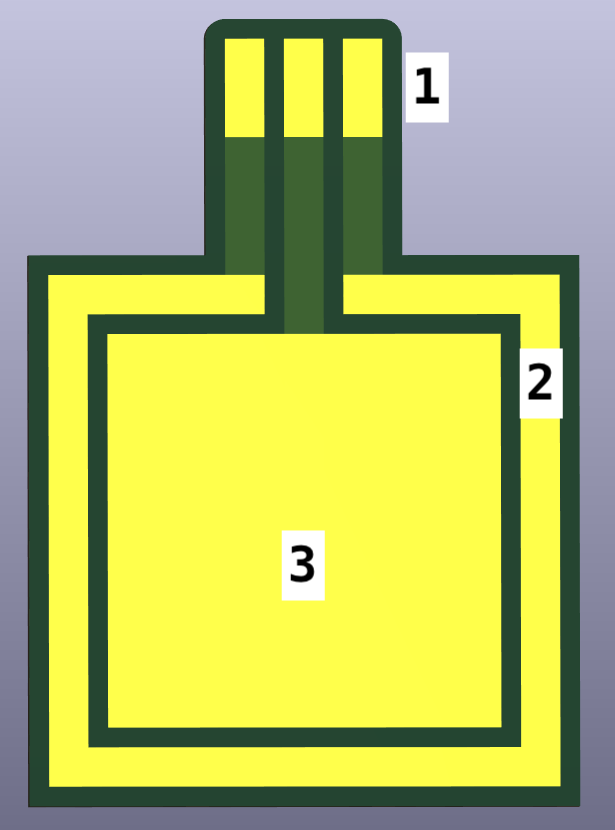
\includegraphics[width=0.6\textwidth]{Figures/GoldElectrode}
\end{minipage}
\begin{minipage}{0.5\textwidth}
    \begin{tabular}{cl} \hline
        1 & \gls{pcb} Connectors \\ \hline
        2 & $2mm$ Fringe Guard \\ \hline
        3 & $20mm \times 20mm$ Main Pad \\ \hline
    \end{tabular}
\end{minipage}
    \caption{The gold electrode \gls{pcb} design.}
    \label{fig:gold-electrode} %chktex 24
\end{figure}

The dimensions of the gold electrodes were chosen to be round values, with the pads having a large surface area and being placed relatively close together.
However, they could not be placed too close together as this could prevent water from effectively flowing between them.
Theoretically, this would reduce the proportion of fringing versus linear current between the electrodes.
This theory is based on the electrical field fringing effect found in capacitors: take two capacitor pads that are placed close together, which experience a certain amount of fringing; if the area of those two pads increases, the quantity of fringing field will increase relative to the side length while the quantity of linear field which would increase relative to the square of the side length~\cite{hegg_capacitor_electric_fringing_2004, sloggett_fringing_fields_in_disc_1986}.

The second method employed to reduce the fringing effect was to keep the resistance between the pads low, which lowers the voltage required to generate a current through the water, which would theoretically further reduce the current fringing.
This theory is also based on capacitors where higher voltages generate stronger electrical fields that spread, or fringe, more.

The gold electrodes were designed with a $20mm \times 20mm$ main pad with a $2mm$ wide fringe guard surrounding it and a spacing between the electrodes of $10mm$.
The expected resistance was then calculated to be between $3,75\Omega$ and $6,25\Omega$ using \refeqn{eqn:conductivity-from-resistance} and conductivity values for salinities between $40$ and $25$ \gls{psu}~\cite{ioc_teos_2010}.

The titanium electrodes were less complicated to design as they only had two variable parameters: their length and spacing.
However, as they were made from titanium wire, the fringing effect between them could not be reduced using the same method as the gold electrodes.
Thus, it was decided to use the gold electrode to evaluate an accurate method for determining conductivity, which could then be applied to the titanium electrodes, where the fringing effect could be mathematically corrected.

The titanium electrodes are significantly more cost-effective than the gold electrodes. 
Thus, if an accurate method for determining salinity using them is developed, they will likely become the primary electrodes of the final device.  
The titanium wire available for this project was $1mm$ in diameter and to account for the unknown resistance between the electrodes, the design allowed for adjustable spacing between the electrodes and adjustable electrode length.

\section{Resistance Measurement Method}

The most common and practical method of measuring resistance is using a resistor divider circuit, which this project chose to employ. 
While current measuring \glspl{ic} exist, the low current ($<1A$) versions use the same resistor divider principle. 
Thus, it was considered to be more cost-effective and configurable to design the resistor divider circuit.

The electrodes were chosen to be the $R_2$ resistor in the voltage divider, and the $R_1$ resistor was chosen to be a significantly larger, known resistance.
The large $R_1$ value allowed a full range of voltages to be applied to the resistor divider while keeping the voltage across the electrodes low, which was advantageous for the reasons mentioned in \refsec{sec:conductivity-electrode-design}.
This configuration also prevented the circuit from being short-circuited if the electrodes were to touch, as the $R_1$ resistor would limit the current.
The voltage drop across the electrodes was then amplified using an op-amp to increase the resolution of the voltage measurement.

\section{Circuit Overview}

The resistor divider circuit was designed to be printed onto a \gls{pcb} (herewith referred to as the probe) manufactured with JLCPCB.
\gls{pcb} manufacturing is cost-effective, has a high precision relative to hand soldering, and the process was familiar to the author, making it the ideal method for creating the prototype.
However, the resistor divider circuit required a few additions to increase its versatility and testing capability, an overview of which is shown in \reffig{fig:circuit-overview}.

\begin{figure}[ht]
    \centering
    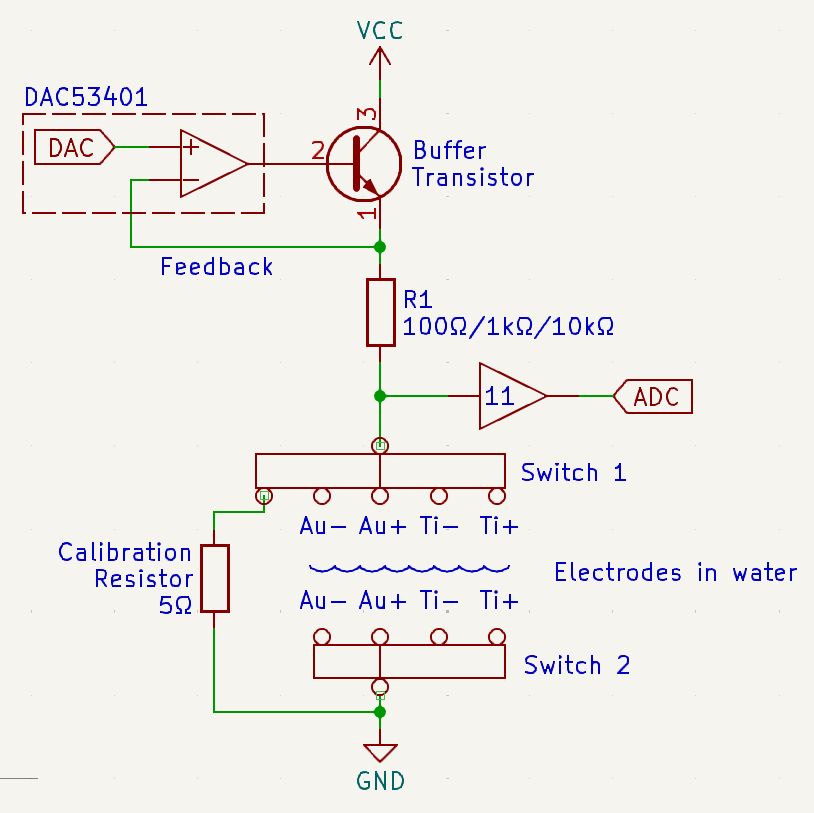
\includegraphics[width=0.6\textwidth]{Figures/CircuitOverview}
    \caption{A simplified representation of the resistance measuring circuit.}
    \label{fig:circuit-overview} %chktex 24
\end{figure}

The voltage driving the resistor divider was provided by a \gls{dac} so that the voltage could be varied and salt water's voltage-resistance relationship could be determined.
The \gls{dac} model was chosen from the \glspl{dac} available on the JLCPCB's website.
The model DAC53401 was ultimately chosen for its high updated time of $10us$ and its advanced functionality, which allowed it to output square, triangle, and sawtooth waves.
This functionality could be used to perform high-frequency tests in addition to linear voltage sweeps.

A typical configuration of a \gls{dac} is to connect its output to the non-inverting input of an op-amp, which would be connected to the base of a transistor.
The transistor's emitter would then be connected to the inverting input of the op-amp.
This configuration allows a higher current to be drawn than the \gls{dac} can provide while maintaining the specified output voltage.
The DAC53401 has an internal op-amp and a feedback input, which allows a transistor to be connected as shown in \reffig{fig:circuit-overview} to achieve the same outcome.

Sets of switches added to the circuit allowed the voltage produced by the \gls{dac} to be directed to an $R_1$ resistor, then across to a pair of electrodes or to a calibration resistor.
The switch model TS3A4751 was chosen from JLCPCB, which contained four switches in its \gls{ic}, as it was very cost-effective for its low and consistent on-state resistance of around $0.7\Omega$.
The circuit required three switching points: one for choosing the $R_1$ resistor, one for choosing the anode and one for choosing the cathode.

It was decided to give the $R_1$ resistor alternate resistances to allow for any possible resistance between the titanium electrodes or unforeseen errors.
The $R_1$ value chosen to pair with the gold electrodes was $100\Omega$ as it was the smallest e12 series resistance that would prevent the board from drawing too much current and burning out the traces or switches.
The final resistances were chosen to be $100\Omega$,  $1k\Omega$ and $10k\Omega$, which would be used when the resistance between the probes was $1\Omega - 10\Omega$, $10\Omega - 100\Omega$ and $100\Omega - 1k\Omega$ respectively.
This configuration allowed for a minimum resolution of $11\%$ of $V_{DAC}$ for the voltage measurement by the \gls{adc} as shown by \refeqn{eqn:adc-resolution}.
\begin{align}\label{eqn:adc-resolution}
 \lfrac{1\Omega}{1\Omega + 100\Omega} * V_{DAC} * 11 = 11\%V_{DAC} \\
 \lfrac{10\Omega}{10\Omega + 100\Omega} * V_{DAC} * 11 = 100\%V_{DAC}
\end{align} 

The anode switch, denoted as switch 1 in \reffig{fig:circuit-overview}, allowed $R_1$ to be connected to any of the four electrodes or to the calibration resistor of $5\Omega$, and the cathode switch, denoted as switch 2 in \reffig{fig:circuit-overview}, allowed any electrode to be connected to ground.
An example of measuring the resistance between the titanium electrodes would be to connect switch 1 to Ti+ and switch 2 to Ti, allowing the voltage drop to be measured.
This configuration also allows current to flow in both directions between electrodes, which can prevent an excessive buildup of chlorine gas or sodium electroplating on the electrodes or electrolysis of the water by taking a resistance measurement in both directions in rapid succession.

To increase the accuracy of the $R_1$ resistors, they were made by placing multiple high-accuracy resistors in parallel, which decreases their resistance uncertainty.
The total uncertainty of the parallel resistance $\delta_{R_{total}}$ is decreased by a factor equal to number of parallel resistors $n$ compared to each resistance's uncertainty $\delta_R$ as shown by \refeqn{eqn:parallel-resistor-total} to \refeqn{eqn:parallel-resistor-uncertainty}.
\begin{gather}
 R_{total} = {\left[ \sum_{i=1}^{n} \lfrac{1}{R} \right]}^{-1} = {\left(\lfrac{n}{R}\right)}^{-1} = \lfrac{1}{n}\cdot R \label{eqn:parallel-resistor-total} \\
 \text{for a function}~f(x_1,x_2,\dots,x_n),~\text{its tolerance} ~\delta_f = \sqrt{\sum_{i=1}^{n} {\left( \lfrac{\partial f}{\partial x_i} \delta x_i \right)}^2} \label{eqn:uncertainty-general-formula} \\
    \therefore \delta_{R_{total}} = \sqrt{{\left( \lfrac{\partial R_{total}}{\partial R} \delta_R \right)}^2} = \sqrt{{\left( \lfrac{1}{n} \delta_R \right)}^2} = \lfrac{1}{n} \delta_R \label{eqn:parallel-resistor-uncertainty}
\end{gather}
The $R_1$ resistors were made from 3 parallel resistors, each with tolerance $\pm1\%$ giving a total tolerance of $\pm0,\bar{3}\%$ and the calibration resistor was made from 4 parallel resistors with tolerance $\pm1\%$ giving a total tolerance of $\pm0,25\%$.

A last switch point was added to the circuit for the gold electrode's fringe guards, an example of which is shown in \reffig{fig:au-measurement-circuit}.
The voltage from $R_1$ was routed to a buffer op-amp with unity gain. 
Its output was then connected to the fringe guard, which effectively repeated the same voltage as the main pad while not affecting any measurements using them.
The other fringe guard could be switched to ground, allowing a current to be generated between the two. 
This current would ideally absorb any possible fringing from the main pads.
The same switch point also allowed the fringe guards to be electrically disconnected to test their effectiveness and to determine if they interfered with the measurement.
Lastly, as the fringe guards held the same voltage difference as the main pads and, in theory, had a higher resistance due to their smaller area, the current flowing between them was assumed to be less than that of the main pads; thus, there was no need to limit the current from the op-amp.

\begin{figure}[ht]
    \centering
    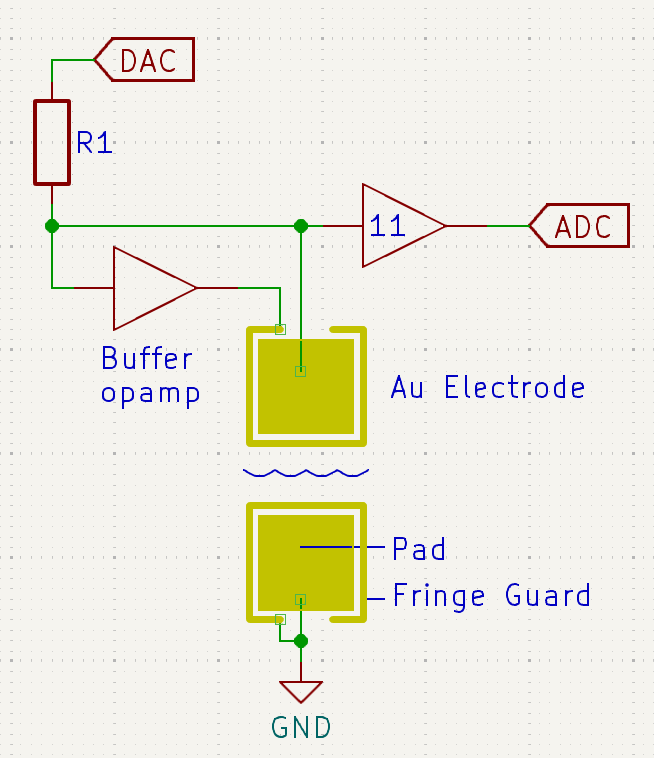
\includegraphics[width=0.4\textwidth]{Figures/AuElectrodeExample}
    \caption{A simplified representation of the resistance measurement circuit using the gold electrodes with the fringe guard.}
    \label{fig:au-measurement-circuit} %chktex 24
\end{figure}

\section{Salinity Calculation and Display}

In order to measure the salinity of the water, the probe \gls{pcb} would be lowered through the ice core hole into the water to capture salinity readings at various depths.
The measurements could either be captured automatically at preprogrammed depth or time intervals or triggered by the user using a controller.
The latter method was chosen for this project because it is a more user-friendly approach, allowing researchers to control precisely which depths the salinity measurements are made and giving them live updates about the probe's status and onboard sensors.

The controller was a straightforward \gls{pcb} with input buttons and rotary switches, two 7-segment displays, a \gls{rs485} communication port and a simple microcontroller.

Saltwater has a high \gls{emi}, which interferes with all wireless communication~\cite{pozzebon_near_field_communication_under_water_2015}.
While high-power wireless communication is viable for ranges up to $70m$, it is more reliable, cost-effective, and power efficient to use a wired connection~\cite{bergmann_wireless_underwater_data_transfer_2013}. 
\gls{rs485} is a robust, long-range embedded communication protocol that only requires a simple \gls{ic} to use, making it ideal for this project.
Additionally, the author was familiar with this protocol and had previous board-to-board communication experience with it.

\Gls{uart} to \gls{rs485} converters are common as most microcontrollers have a \gls{uart} communication port.
This project used half-duplex \gls{rs485} as it is the industry standard, and it is more cost-effective than full-duplex \gls{rs485}, which requires an additional \gls{uart} to \gls{rs485}.

The microcontroller was chosen from the STM32F030 series as it did not need to perform any complex calculations, and the author was familiar with this series.

With an external controller, a waterproofed probe could be lowered into the water to measure its salinity.
The chosen method of waterproofing the probe was to coat it with epoxy resin, as this was the most familiar and cost-efficient method available.
The other notable option is to create a waterproof housing for the probe, but this can be complex and expensive.
In addition to the circuitry shown in \reffig{fig:circuit-overview}, the probe had a temperature and depth sensor, which are discussed in \refsec{sec:temp-depth-measurement}, an \gls{rs485} communication port and a microcontroller.
The microcontroller was chosen from the STM32F4 series as it is the most cost-effective series with a \gls{fpu}, allowing the salinity to be calculated on board as per the equations in \refsec{sec:salinity-conductivity-relationship}.


\section{Temperature and Depth Measurement}\label{sec:temp-depth-measurement}

Waterproof depth sensors were too expensive for this project's budget, costing around $\$100$.
An alternative approach is to use a non-waterproof pressure sensor that is isolated from the water using a flexible membrane that allows the external pressure to be transmitted to the sensor.
The WF183DE pressure sensor was chosen as it was the most cost-effective sensor rated for above 50 meters of water pressure available at \texttt{JLCPCB}.
Should this approach fail, the backup plan was to use the controller to manually input a depth so that the salinity could still be calculated.

The temperature sensor was an arbitrarily chosen surface-mount sensor with high accuracy of $\pm 0,3\degree C$ and a wide temperature range of $-45$ to $130\degree C$.
Epoxy resin is a poor thermal conductor~\cite{epotek_thermally_conductive_epoxies}. 
Thus, the temperature sensor should be coated with a very thin layer of epoxy when the probe \gls{pcb} is cast, allowing for a more accurate measurement.
The choice of microcontroller and pressure sensor also provided this board with two alternative temperature sensors, which were less accurate but could be used in the event that the primary temperature sensor failed.